\section{Related work}\label{sec:rel}
In this section, we survey previous work and focus on the most relevant pieces.
Section~\ref{sec:trajvisana} and ~\ref{sec:interactive} summarize the related works in trajectory visual analysis and interactive data visualization for large dataset, respectively.

\subsection{Trajectory visual analysis}\label{sec:trajvisana}
Trajectory is the most common representation of the object movement.
Each trajectory consists of a sequence of spatial locations (i.e., GPS points).
To support the understanding and analyzing of the trajectory dataset,
many visualization and visual analytics systems are proposed and implemented in literature.
As stated in~\cite{chen2015survey}, existing trajectory visual analysis techniques can be classified into three categories according to visualization form,
i.e., point-based visualization, line-based visualization and region-based visualization, respectively.
We briefly introduce the research works in these three categories, and refer the interested readers to a recent survey~\cite{chen2015survey} for detail discussions.

The point-based visualization captures the spatial distribution overview of the GPS points in the trajectories of moving objects.
Many density-based methods, e.g., kernel density estimation, are applied in point-based visualization methods~\cite{liu2013vait,yang2016exploring,chae2014public,xie2008kernel, borruso2008network}.
These point-based visualization methods alleviate the visual clutter in large amount data by sacrificing the detail information of trajectories, e.g., the sequence order of GPS points.
However, the point-based visualization result cannot identify the movement of the individual object and reveal the moving details, e.g., path, direction and origin-destination ~\cite{chen2015survey}.
The region based visualization approaches divide the whole region into sub-regions in advance,
then visualize the traffic situation in each sub-region.
These methods visualize the macro-pattern very well as it leverages different aggregation techniques~\cite{guo2009flow,wood2010visualisation,von2015mobilitygraphs}.
In this work, we focus on the line-based visualization methods, which are widely used in visual analysis applications.
It uses polylines to show the trace of the object movements.
Through this, it preserves the continuous of the objects moving information~\cite{guo2011tripvista,hurter2009fromdady}.
However, the line-based visualization methods suffer serious visual clutter due to the cross of the polylines in the large amount of the trajectories.
To alleviate this problem, many clustering techniques are proposed in the virous visual analysis with different trajectory datasets, e.g., flight ~\cite{ferreira2013vector}, taxi trips~\cite{rinzivillo2008visually} and hurricane trajectories~\cite{andrienko2017clustering}.
Moreover, advanced interaction techniques~\cite{kruger2013trajectorylenses, ferreira2013visual} and edge bundling techniques~\cite{zeng2019route} are also devised to detect the movement patterns.
Unlike existing line-based visualization techniques, we propose a visual fidelity  guaranteed sampling approach for line-based trajectory visualization with large-scale input data.
To the best of our knowledge, it is the first work which offers theoretical visual fidelity guaranteed of the sampling result for line-based trajectory visualization.





\subsection{Interactive visualization for large dataset}\label{sec:interactive}

With the technology advance of location-acquisition device, the size of trajectory dataset becomes extremely huge recently.
For example, the operating taxis in Shenzhen generates 9.3GB trajectory data per day.
Due to the limited rendering ability of modern commodity graphics device, generating visualizations for such scale of dataset always take considerable amount of time, 
or even impractical in practice~\cite{park2016visualization}.
In literature, many works are proposed to achieve interactive visualization in large dataset (not only for trajectory dataset), we briefly elaborate the most representative pieces in this subsection.

\begin{figure}
	\centering
	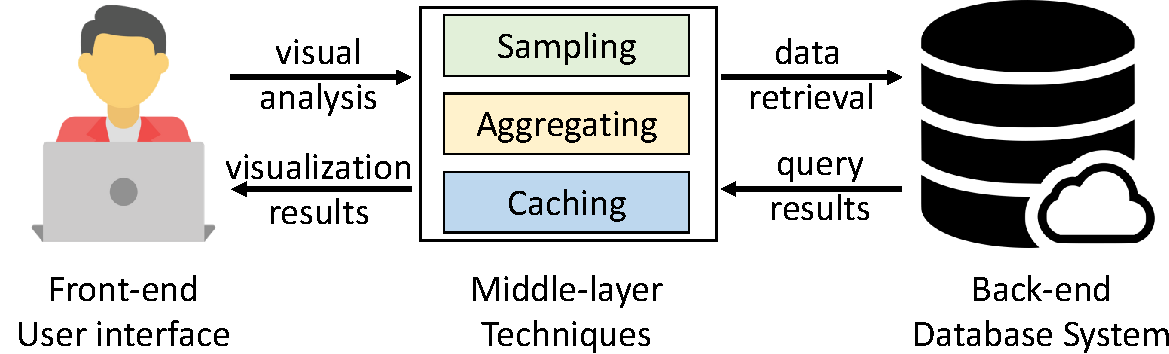
\includegraphics[width=0.45\textwidth]{pictures/framework/framework.pdf}
	\caption{Interactive visualization system architecture for large dataset}
	\label{fig:framework}
\end{figure}

Figure~\ref{fig:framework} illustrates the architecture of interactive visualization systems (e.g., Spotfire~\footnote{\url{https://www.tibco.com/products/tibco-spotfire}}, Tableau~\footnote{\url{https://www.tableau.com/}}) for large-scale datasets.
It consists of three layers: the user interface in front-end, the optimization techniques in middle-layer, and the (cloud-based) database management system in the back-end.
Typically, the researchers in visualization community focused on improving the information visualization effectiveness at the front-end, 
e.g., designing novel visualization techniques to assist data analysts to obtain data insight easily (D3~\footnote{\url{https://d3js.org/}}).
For the researchers in database community, they are working on the efficiency aspect for large data processing,
e.g., devising big data processing systems and techniques for efficient query processing at back-end (Spark~\footnote{\url{https://spark.apache.org/}}).
In recent year, both visualization and database communities are dedicating to advance the techniques in interactive visual analysis for large-scale dataset,
for example, the optimization techniques in the middle-layer (see Figure~\ref{fig:framework}).
We then briefly elaborate these techniques in middle-layer in subsequent as they are relevant to our technqiues in this work.

\stitle{Aggregating-based techniques}
Aggregating-based optimization techniques~\cite{zeng2013visualizing,von2015mobilitygraphs} in the middle-layer provide interactive visualization analysis for large-scale data by 
reducing the number of rendering data via preprocessing them by aggregators (e.g., clustering).
Returning to the trajectory visual analysis, the aggregating techniques can be further distinguished by how to generate the spatial partitions.
For example, OD Map~\cite{wood2010visualisation} divides the whole map into nested uniform grid, and uses the color of a grid to present the flow magnitude.
\cite{guo2009flow} employs the hierarchical administrative regions as basic units and visualize the flow by linking different units.
Instead of using static predefined spatial partitions in ~\cite{wood2010visualisation,guo2009flow},
\TB{MobilityGraph~\cite{von2015mobilitygraphs} visualizes the aggregated twee posts locations in these regions which are defined by a spatial graph clustering algorithm dynamically.}
Our problem and solution approaches are different from these research works as we focused on visualizing the raw input data, instead of the aggregation results.
% by the movement patterns.


\stitle{Sampling-based techniques}
Sampling is a delta-facto solution for the interactive visualization problems with large-scale input data.
It is widely studied in both visualization and database communities, e.g., ~\cite{battle2013dynamic,chen2014visual,park2016visualization}, 
In particular, ~\cite{chen2014visual} devised an sampling algorithm to preserve the meaningful data items according to the analyzing requirement such as the multi-class data analysis and hierarchical exploration. 
\TB{In addition, the usage of others visual channels of the points, e.g., color and size and opacity are discussed in it~\cite{chen2014visual,woodruff1998constant}}.
The most relevant work of ours in literature is~\cite{park2016visualization}, which designed for the scatter plot and aim to not only solve the overdrawing of the points but also try to preserve the information distribution of the original dataset.
Specifically, they formulated a loss function which evaluates the visual loss of the sampling result effectively,
they validate the proposed method based on three common visualization tasks, e.g., regression, density estimation and clustering.
However, the techniques in~\cite{park2016visualization} cannot be adapted to our large-scale trajectory visualization problem
as (i) the complexity of the trajectories~\cite{pelekis2010unsupervised}, and (ii) the loss function and the loss-function based solution is specified for scatter points, not applicable for trajectories.
For trajectory visual analysis,  most of the existing trajectory sampling techniques (if not all) cluster the trajectories at first, 
then select the most representative trajectories from each cluster and visualize them.
It is impractical to provide interactive visualizations for real-world applications as 
(i) the trajectory similarity calculation and clustering algorithms are expensive~\cite{pelekis2007similarity},
and (ii) the trajectory clustering is still an open problem in both communities~\cite{panagiotakis2011segmentation,agarwal2018subtrajectory}.
Unlike the above research works, in this paper, we propose a visual fidelity guaranteed sampling approach ($\vats{}$) for the large-scale trajectory visualization problem,
we demonstrate the superiority of our proposal by both case- and user- studies in real world applications.
% Some techniques further focus on the clustering and sampling of trajectory segments instead of the whole trajectories.


%A good visualization-aware sampling strategy should reduce the data size as much as possible and sacrifice the visual fidelity as less as possible.




\stitle{Caching-based and other techniques}
Caching is commonly used to improve the performance of large-scale data processing system, e.g., search engine~\cite{xu2015diversified}.
Chan et al. present ATLAS~\cite{chan2008maintaining} which utilizes caching techniques for the efficient data communication between server and client.
In addition, it also exploits the powerful multi-core server to accelerate analysis task processing from the middle-layer to the back-end.
Piringer et al.~\cite{piringer2009multi} propose a multi-threading architecture for the interactive visual exploration,
which takes advantages of multi-core devices and avoids the multi-threading pitfalls to provides quick visual feedback.
However, our proposed techniques in this work are orthogonal to the researches in this category.



%Current advancing sampling techniques in the visualization domain are mostly 
%Some works design advanced sampling algorithms to preserve the meaningful data items according to the analyzing requirement such as the multi-class data analysis and hierarchical exploration~\cite{chen2014visual}. Furthermore, to the usage of more visual channels of the points other than location such as color~\cite{chen2014visual}, size~\cite{woodruff1998constant} and opacity are discussed.
%Closely related to our work, Park et al.~\cite{park2016visualization} proposed the visualization-aware techniques for the scatter plot. 
%
%In comparison with the sampling techniques for scatter plot, the trajectory sampling is more challenging because of the complexity of the trajectories~\cite{pelekis2010unsupervised}. 
%
%
%Many exiting visual analytics systems leverage powerful database manage system as the backend to facilitate the fast data processing. Based on the solution proposed in ScalaR~\cite{battle2013dynamic}, a common visualization framework involving sampling technique is illustrated as Figure~\ref{fig:framework}, where a sampling layer is set between the backend and frontend. Since the sampling methods are always designed for complicated task, the algorithms may not be efficient enough to support the interactive data exploration. Thus the cache model is always implemented to save the sampling results. In our scenario, the users query large amount of data(e.g. all Shenzhen trajectories in one week) once and then conduct interactive multi-resolution exploration based on the sampled data, thus the method need to guarantee the visual quality well across different resolutions.
%
%Sampling is a delta-facto solution for the problems with big data. Target at the sampling requirement, the naive solutions such as uniform random sampling cannot generate acceptable because the serious visual information loss. In this section, we first define a loss function to evaluate the visual quality between the visualization results between whole dataset and sampled subset. Then we analyze the hardness of the problem and design algorithms for it.
%
%
%\begin{figure}[t]
%	\centering
%	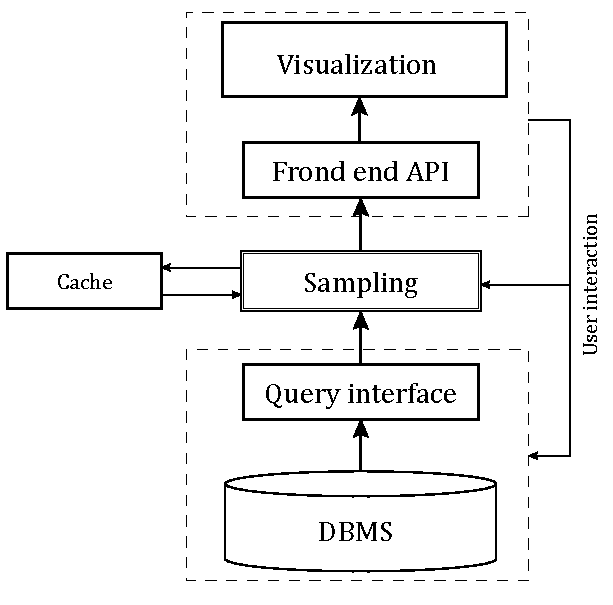
\includegraphics[width=0.3\textwidth]{pictures/framework/DBVAframework.pdf}
%	\vspace{-5mm}
%	\caption{A visualization framework involving sampling layer between the front-end and database management system.}
%	\vspace{-5mm}
%	\label{fig:framework}
%\end{figure}
%
